\documentclass{article}
\usepackage[utf8]{inputenc}
\usepackage[english]{babel}
\usepackage[font=small,labelfont=bf]{caption}
\usepackage{geometry}
\usepackage{natbib}
\usepackage{pxfonts}
\usepackage{graphicx}
\usepackage{newfloat}
\usepackage{setspace}
%\doublespacing

\newcommand{\argmax}{\mathop{\mathrm{argmax}}\limits}

\title{\textit{Supplementary materials for: } High-level cognition
  during story listening is reflected in high-order dynamic
  correlations in neural activity patterns} \author{Lucy
  L. W. Owen$^1$, Thomas H. Chang$^{1,2}$, and\
  Jeremy R. Manning\textsuperscript{$1, \dagger$}\\
  [0.1in]$^1$Department of Psychological and Brain
  Sciences,\\Dartmouth
  College, Hanover, NH\\
  $^2$Amazon.com, Seattle, WA\\
  \textsuperscript{$\dagger$}Address correspondence to
  jeremy.r.manning@dartmouth.edu}

\bibliographystyle{apa}

\begin{document}
\maketitle

\setcounter{equation}{0}
\setcounter{figure}{0}
\setcounter{table}{0}
\setcounter{page}{1}
\setcounter{section}{0}
\makeatletter
\renewcommand{\theequation}{S\arabic{equation}}
\renewcommand{\thefigure}{S\arabic{figure}}
\renewcommand{\bibnumfmt}[1]{[S#1]}
\renewcommand{\citenumfont}[1]{S#1}



\begin{figure}[tp]
\centering
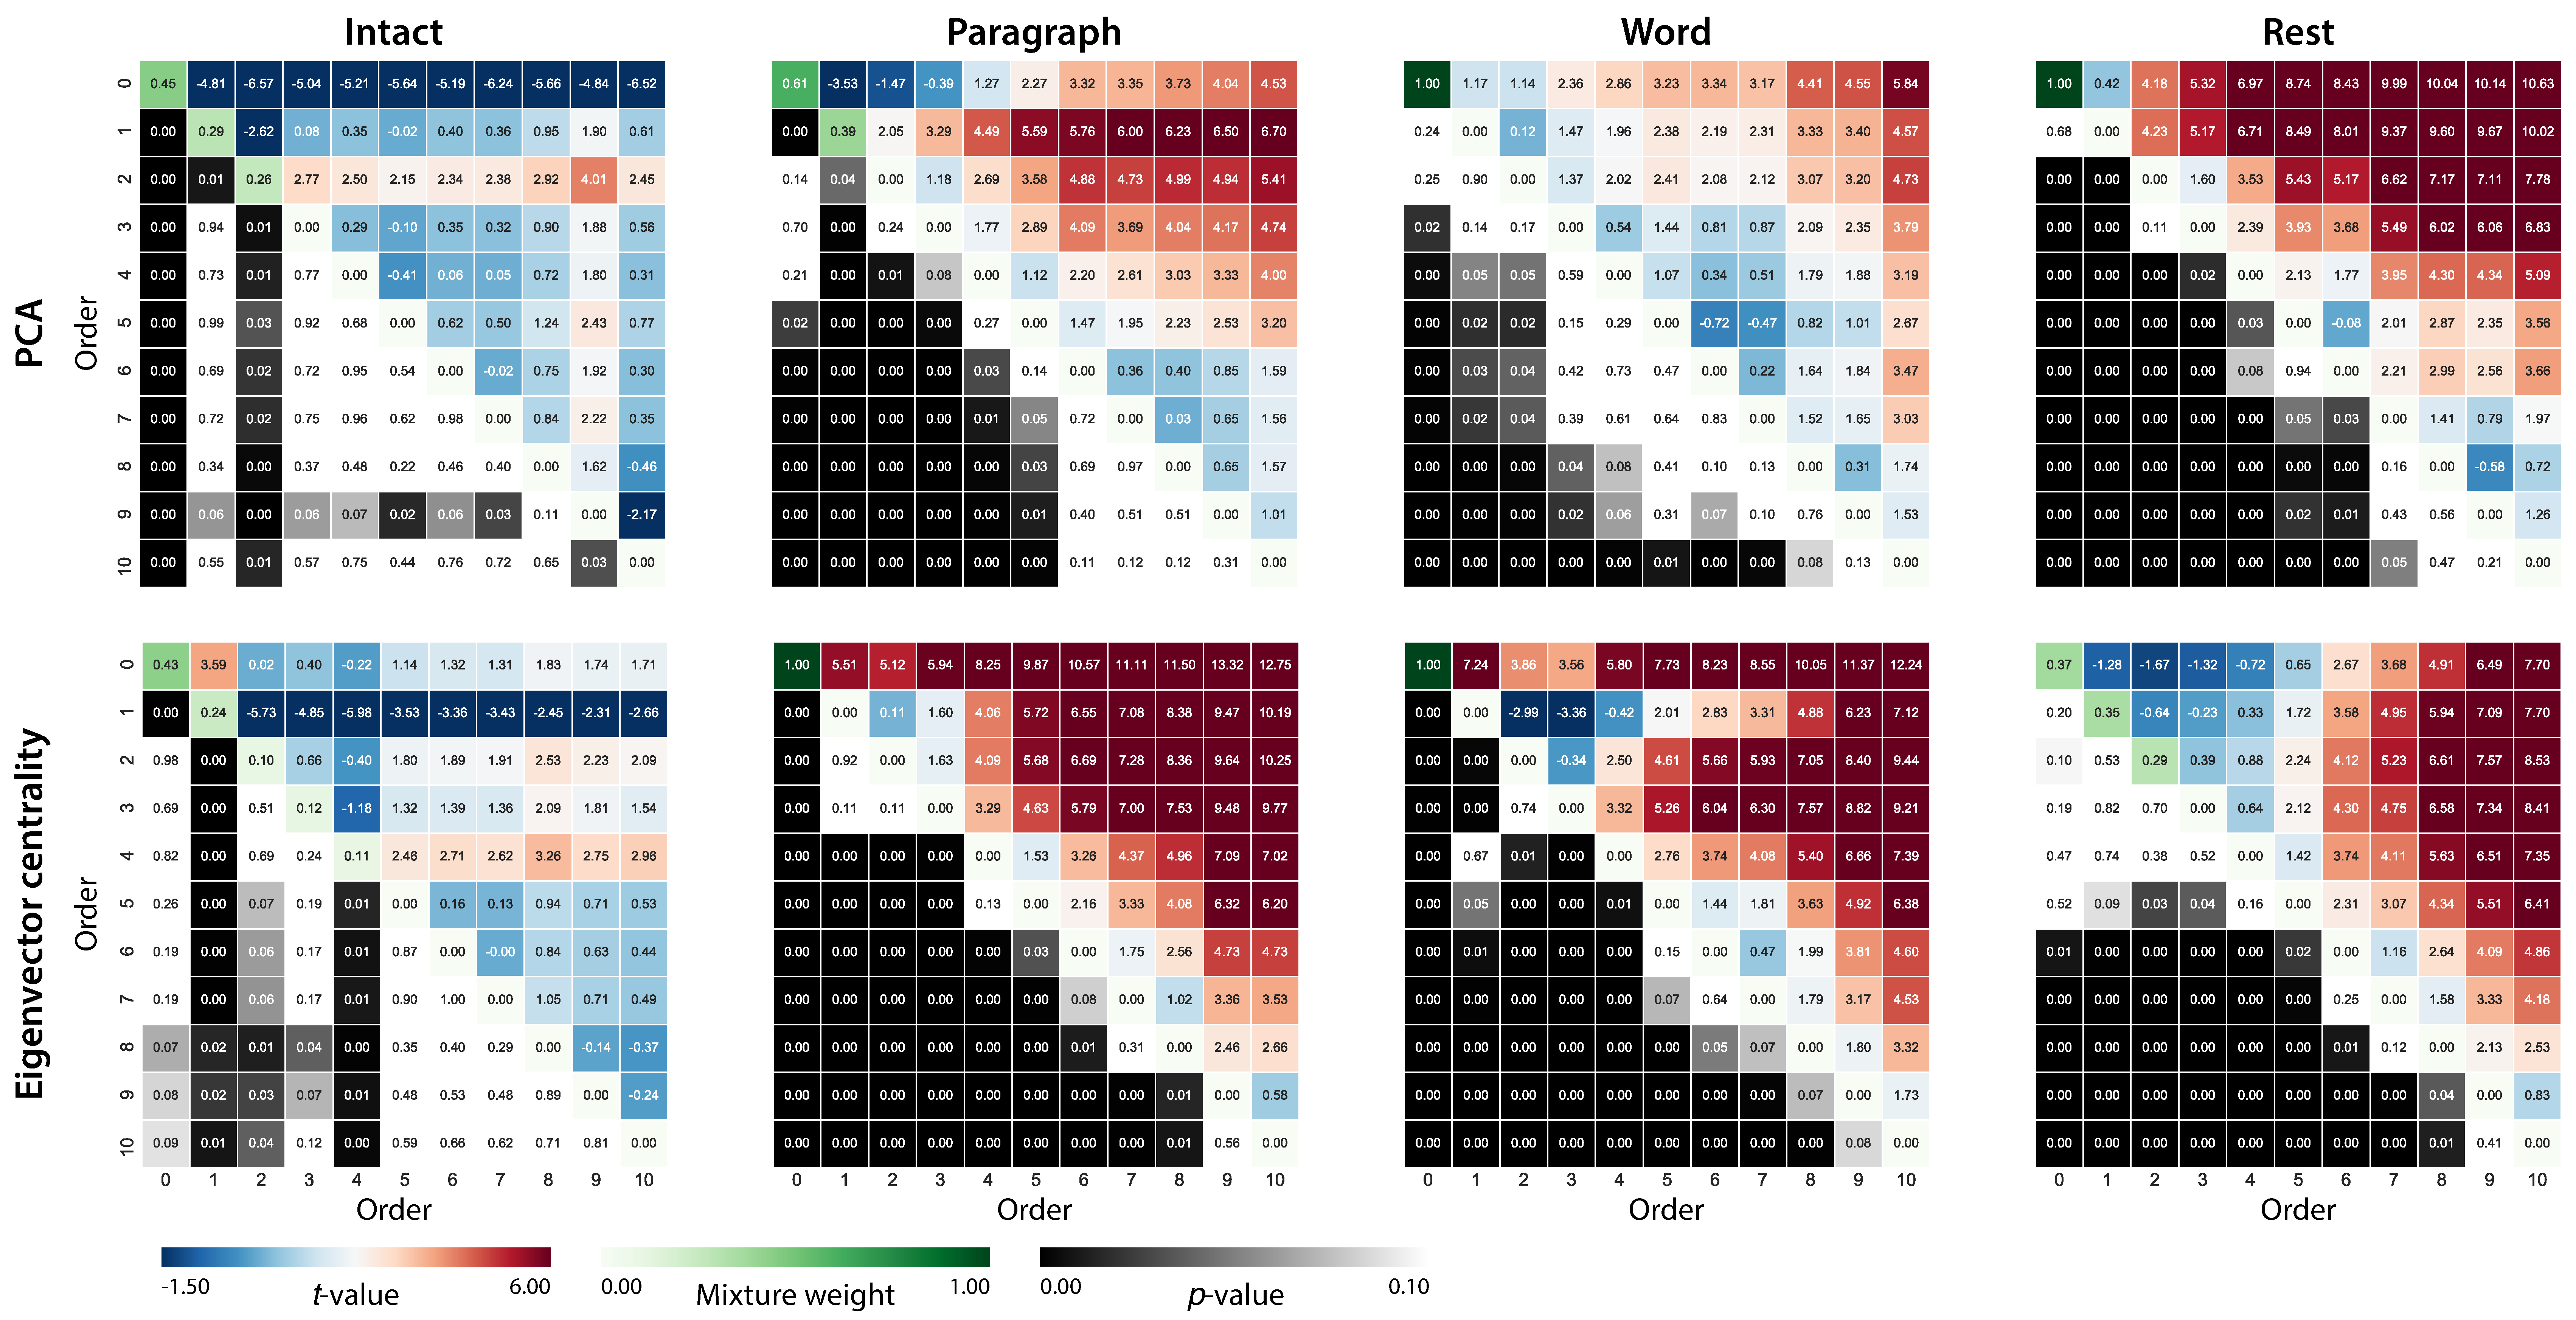
\includegraphics[width=1\textwidth]{figs/stats_heatmaps}
\caption{\textbf{Statistical summary of decoding accuracies for
    different neural features.}  Each heatmap displays decoding
  results for one experimental condition (intact, paragraph, word, and
  rest).  We considered dynamic activity patterns (order 0) and
  dynamic correlations at different orders (order $> 0$).  We used two-tailed $t$-tests to compare the
  distributions of decoding accuracies obtained using each pair of
  features.  The distributions for each feature reflect the set of
  decoding accuracies obtained 

  In the upper triangles of each map, warmer colors (positive $t$-values) indicate that the
  neural feature indicated in the given row yielded higher accuracy than the
  feature indicated in the given column.  Cooler colors (negative
  $t$-values) indicate that
  the feature in the given row yielded lower decoding accuracy than
  the feature in the given column.


  The upper triangles of each heatmap report the $t$-values
  from a 



  \textbf{Heatmaps conveying statistical results comparing decoding
    accuracy for each order.}  For each condition (intact, paragraph
  scrambled, word scrambled, and rest) and for each reduction
  technique (PCA and eigenvector centrality), we compared the
  distribution of decoding accuracy for each order. The upper triangle
  of each heatmap conveys the results of t-tests, and the lower
  triangle conveys corresponding p-values.  The diagonal is the
  results of the optimization of the phi parameter. }
\label{fig:stats_heatmaps}
\end{figure}

\begin{figure}[p!]
\centering
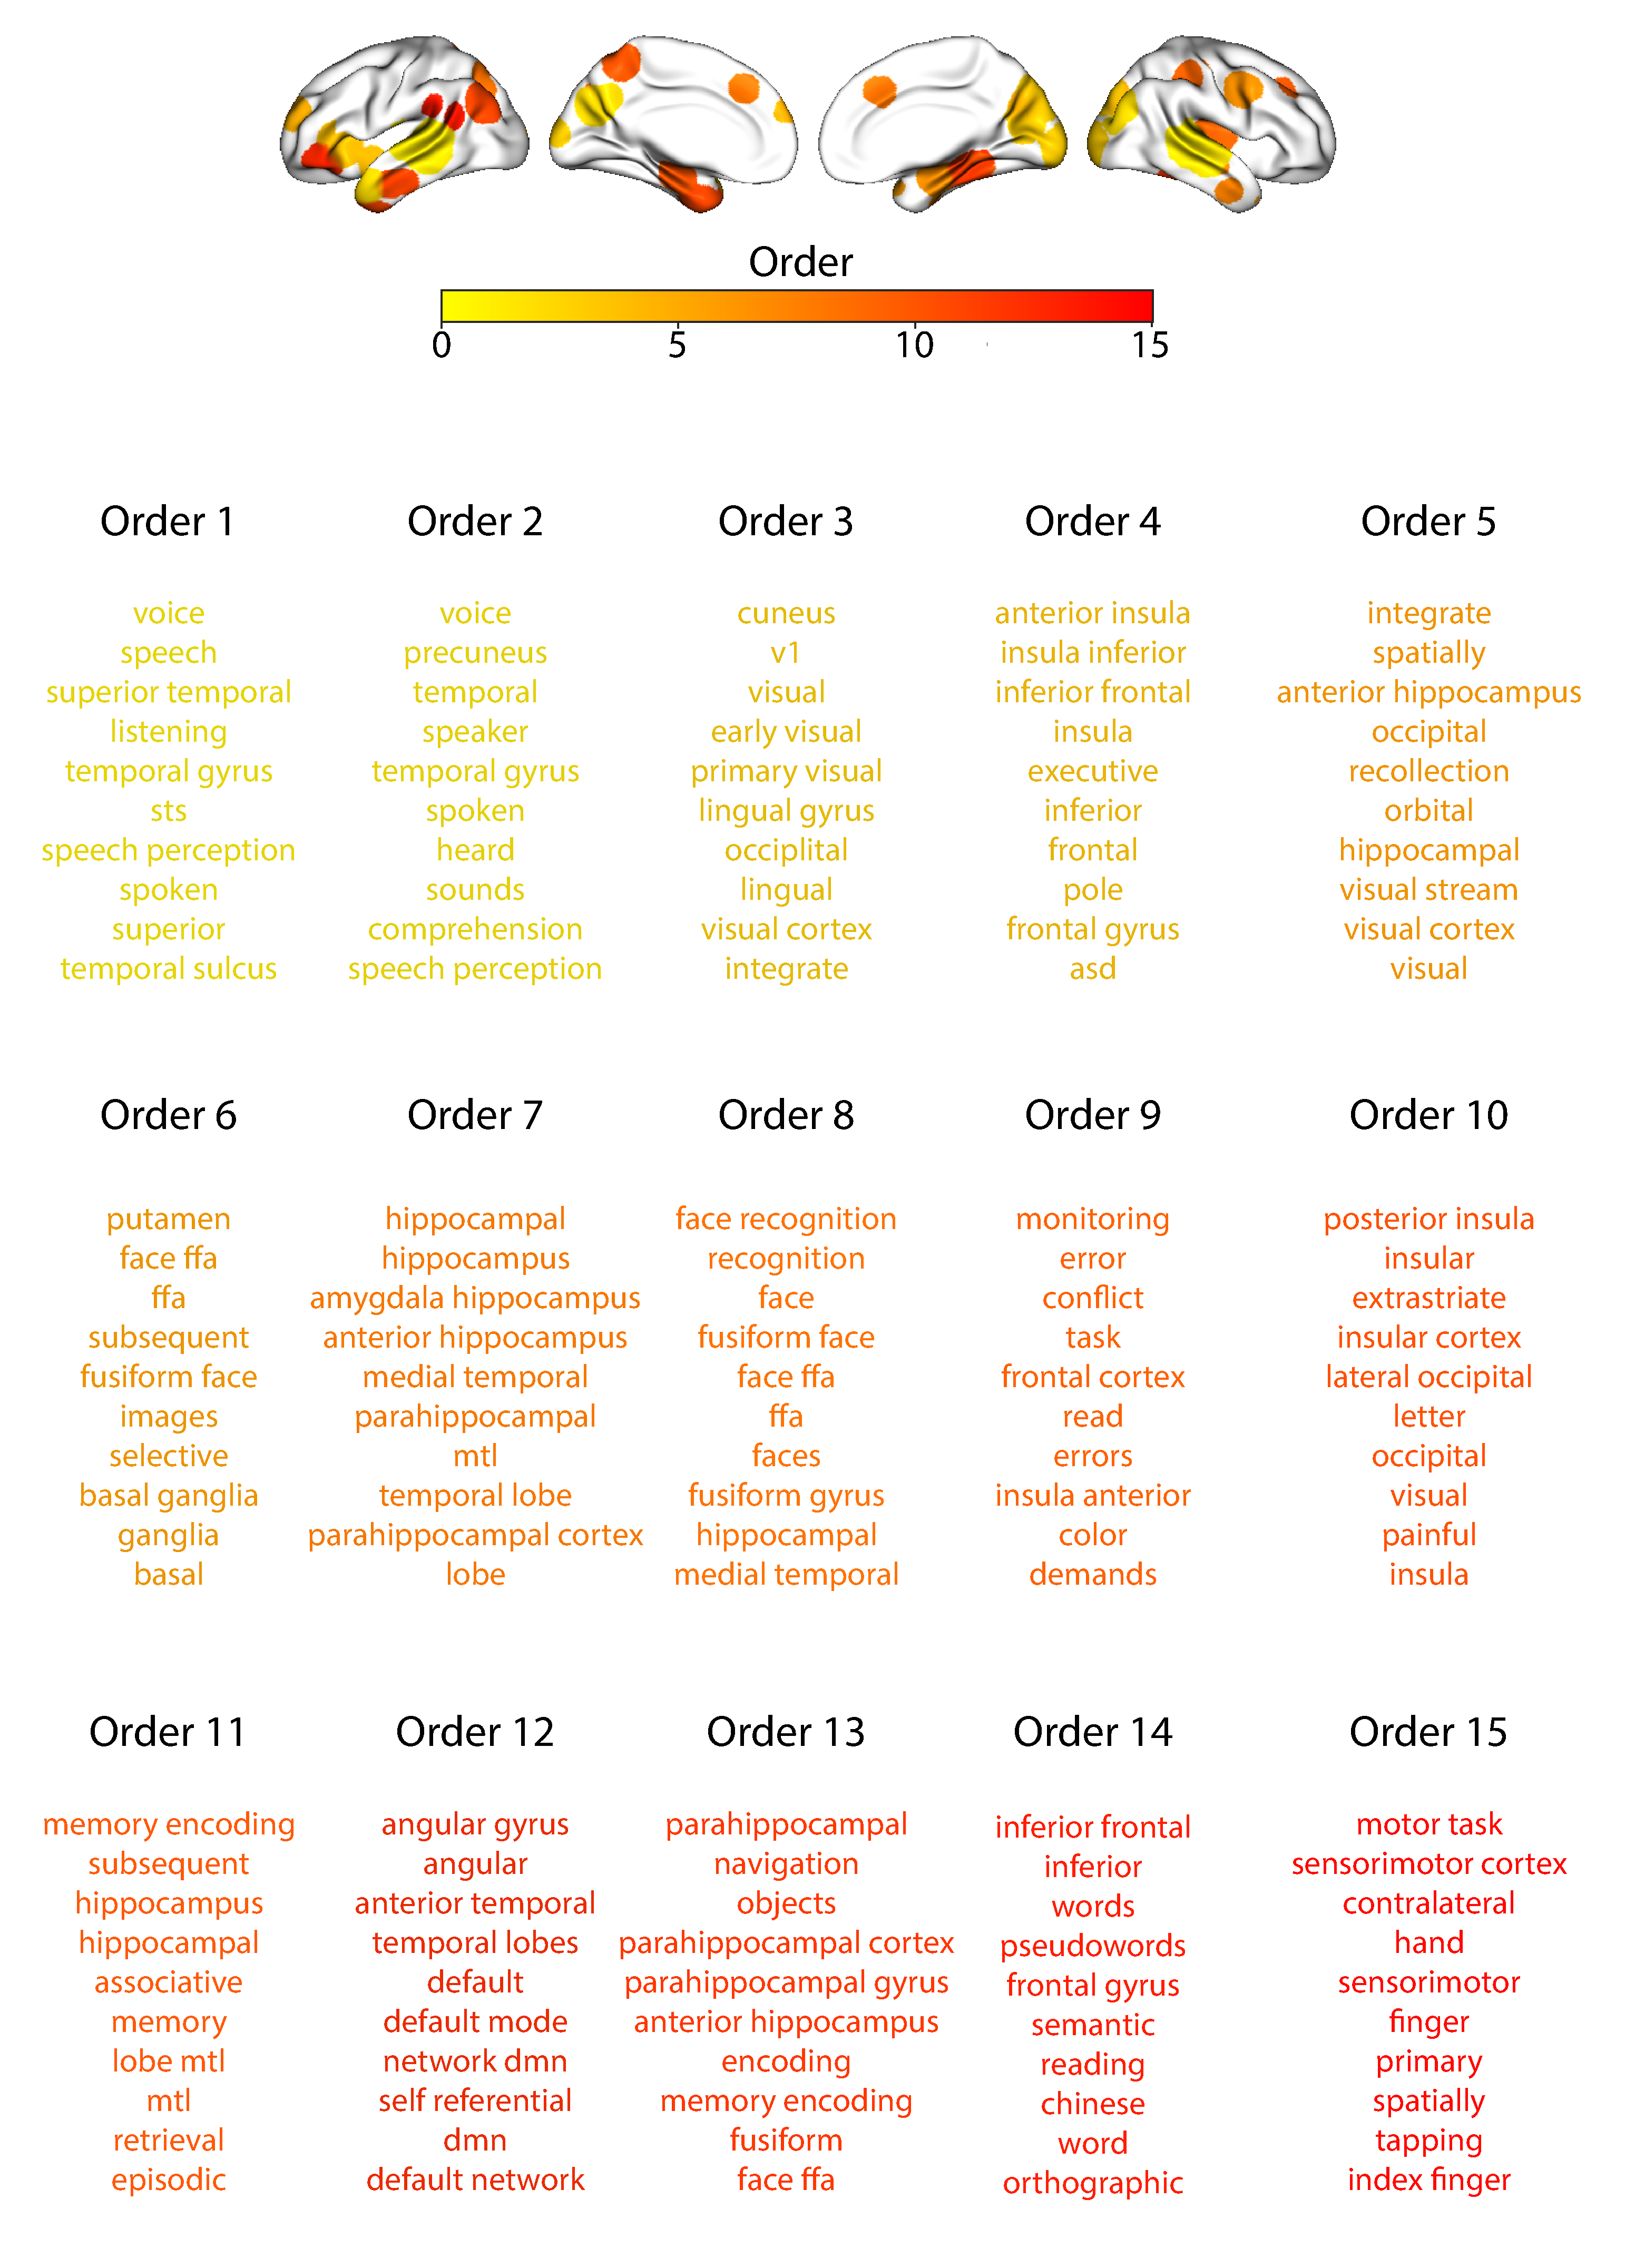
\includegraphics[width=0.75\textwidth]{figs/supp_15_intact}
\caption{\textbf{Top 10 terms associated with the endpoints of the
      strongest correlations for the intact experimental condition.}  Each color corresponds to orders 1-15 of
    inter-subject functional correlations. The inflated brain plots
    display the locations of the endpoints of the 10 strongest
    (absolute value) correlations at each order, projected onto the
    cortical surface~\citep{CombEtal19}.  The lists of terms on the
    right display the top 10 Neurosynth terms~\citep{RubiEtal17}
    decoded from the corresponding brain maps for each order for the intact condition.}
\label{fig:intact}
\end{figure}

\begin{figure}[p!]
\centering
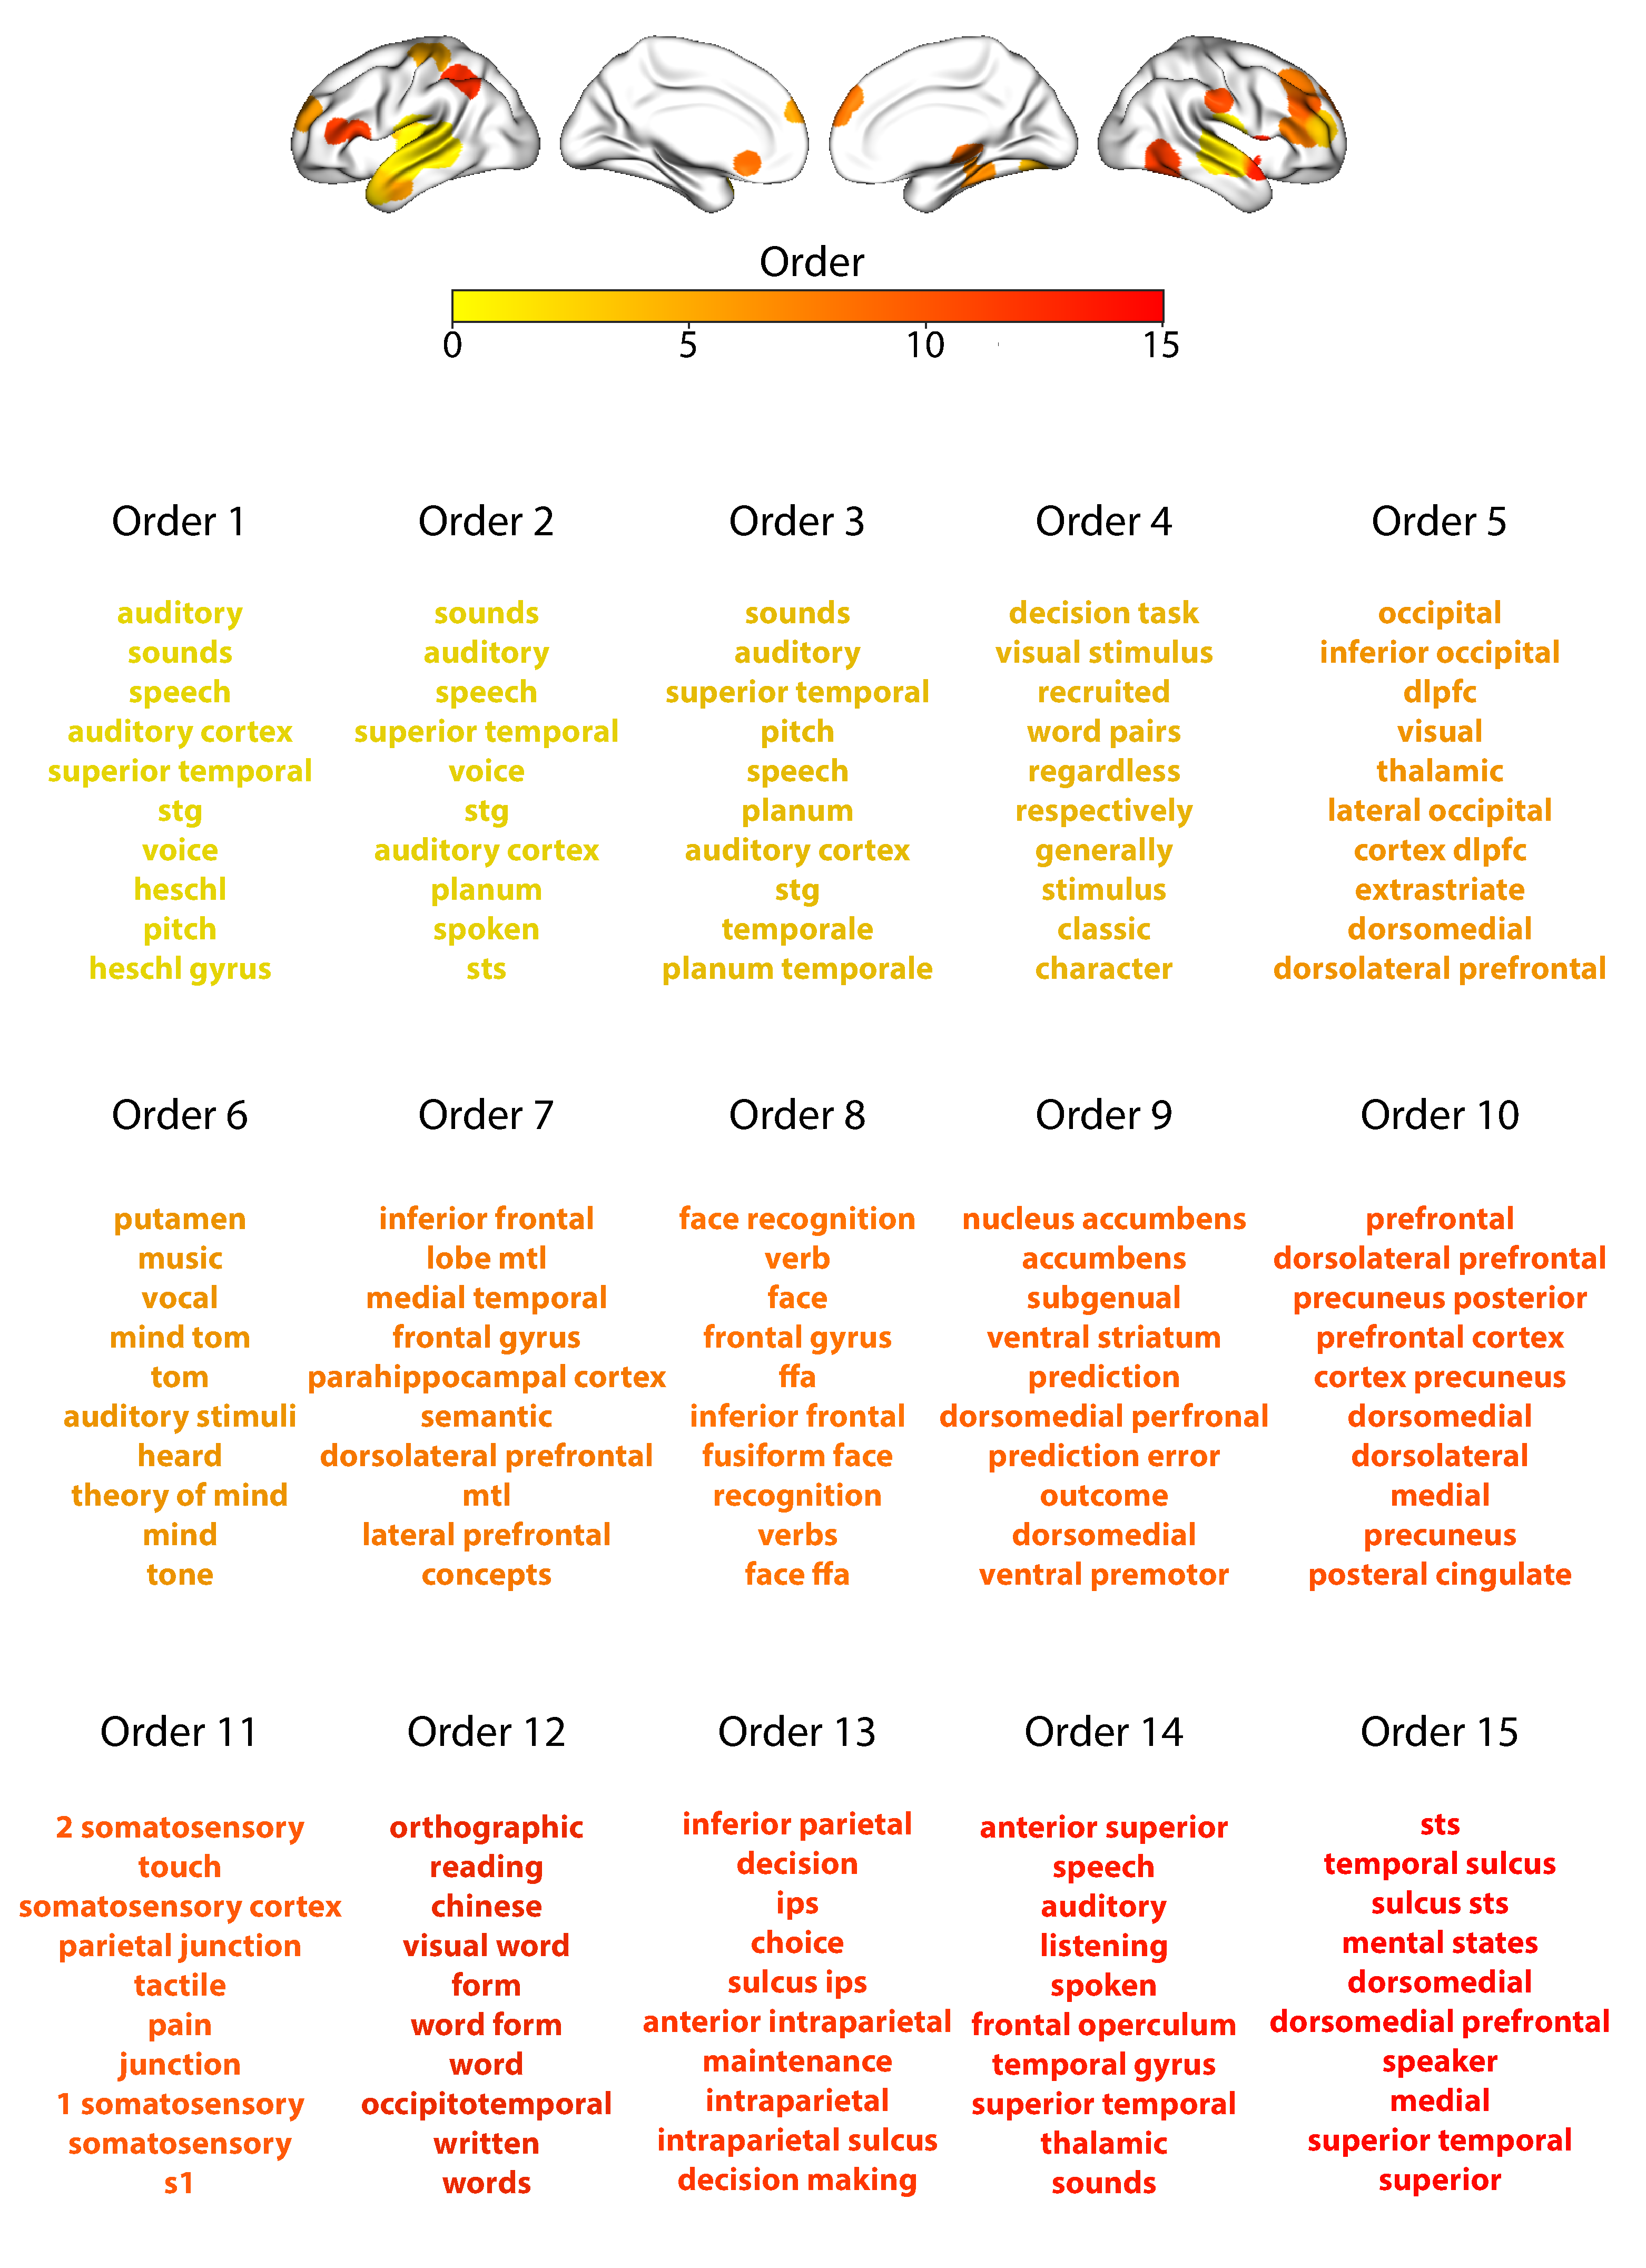
\includegraphics[width=0.75\textwidth]{figs/supp_15_paragraph}
\caption{\textbf{Top 10 terms associated with the endpoints of the
      strongest correlations for the paragraph scrambled condition.}  Each color corresponds to orders 1-15 of
    inter-subject functional correlations for the paragraph scrambled condition. The inflated brain plots
    display the locations of the endpoints of the 10 strongest
    (absolute value) correlations at each order, projected onto the
    cortical surface~\citep{CombEtal19}.  The lists of terms on the
    right display the top 10 Neurosynth terms~\citep{RubiEtal17}
    decoded from the corresponding brain maps for each order.}
\label{fig:paragraph}
\end{figure}

\begin{figure}[p!]
\centering
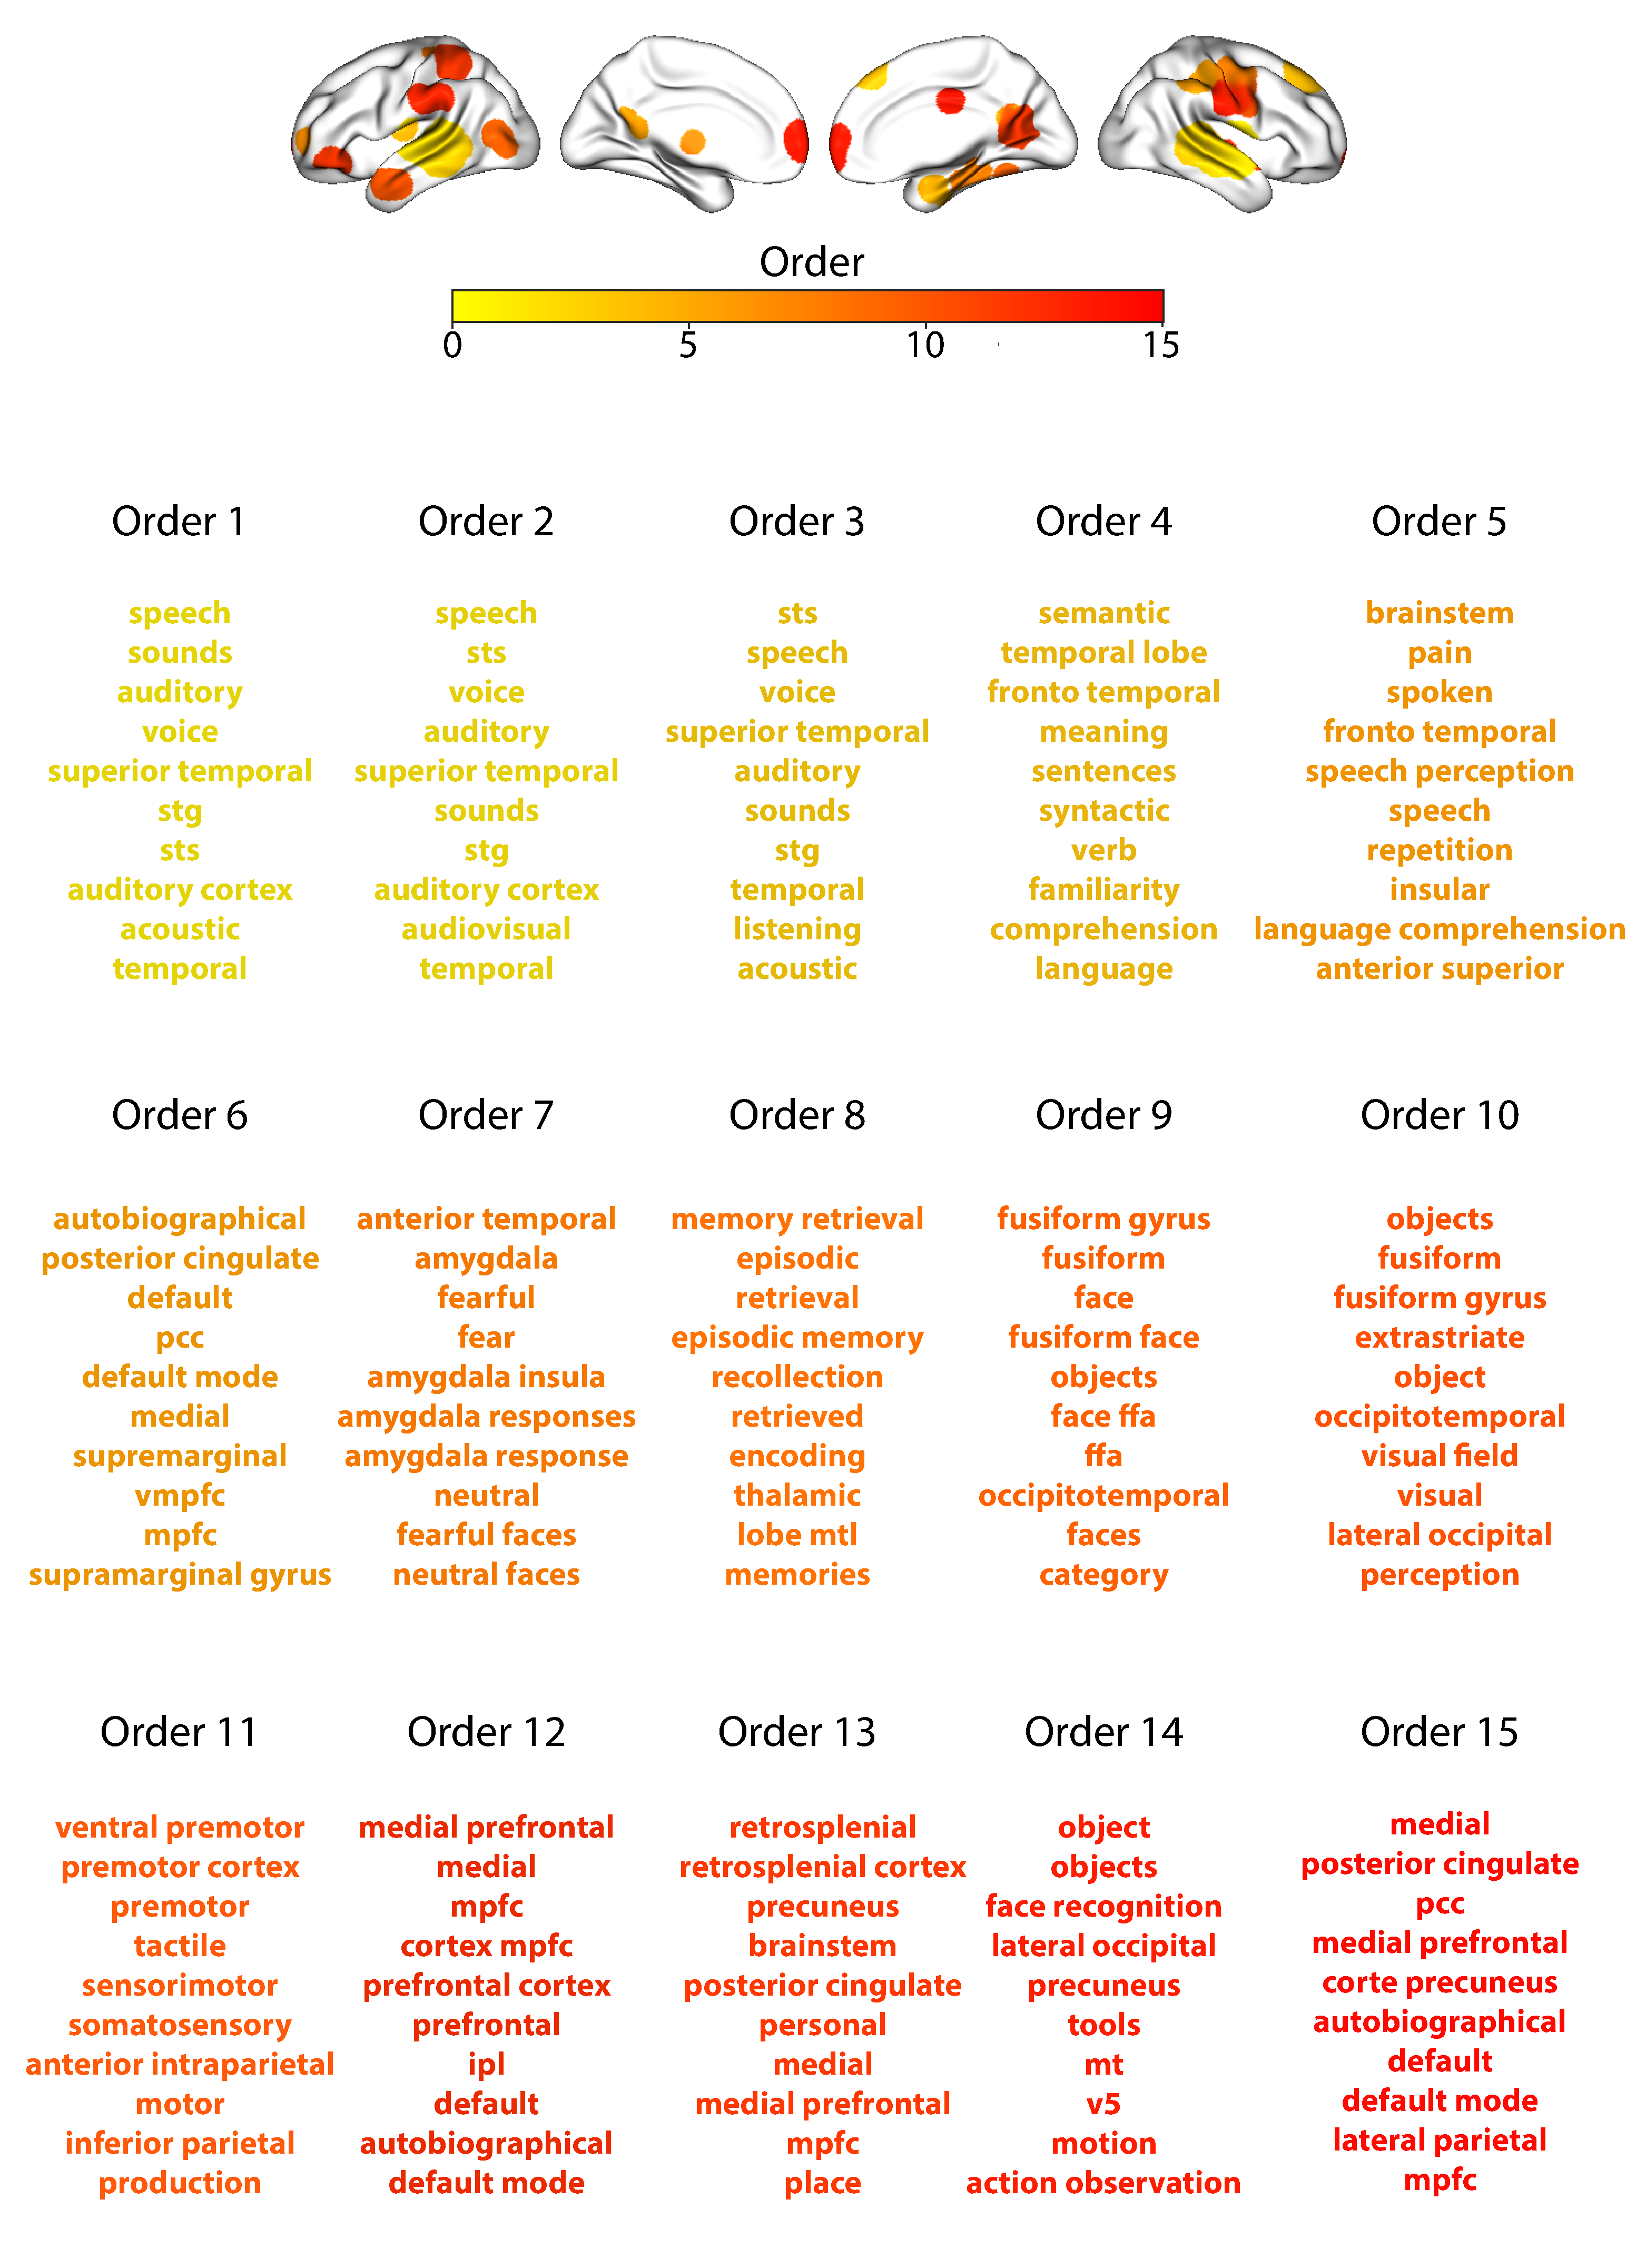
\includegraphics[width=0.75\textwidth]{figs/supp_15_word}
\caption{\textbf{Top 10 terms associated with the endpoints of the
      strongest correlations for the word scrambled condition.}  Each color corresponds to orders 1-15 of
    inter-subject functional correlations for the word scrambled condition. The inflated brain plots
    display the locations of the endpoints of the 10 strongest
    (absolute value) correlations at each order, projected onto the
    cortical surface~\citep{CombEtal19}.  The lists of terms on the
    right display the top 10 Neurosynth terms~\citep{RubiEtal17}
    decoded from the corresponding brain maps for each order.}
\label{fig:word}
\end{figure}

\begin{figure}[p!]
\centering
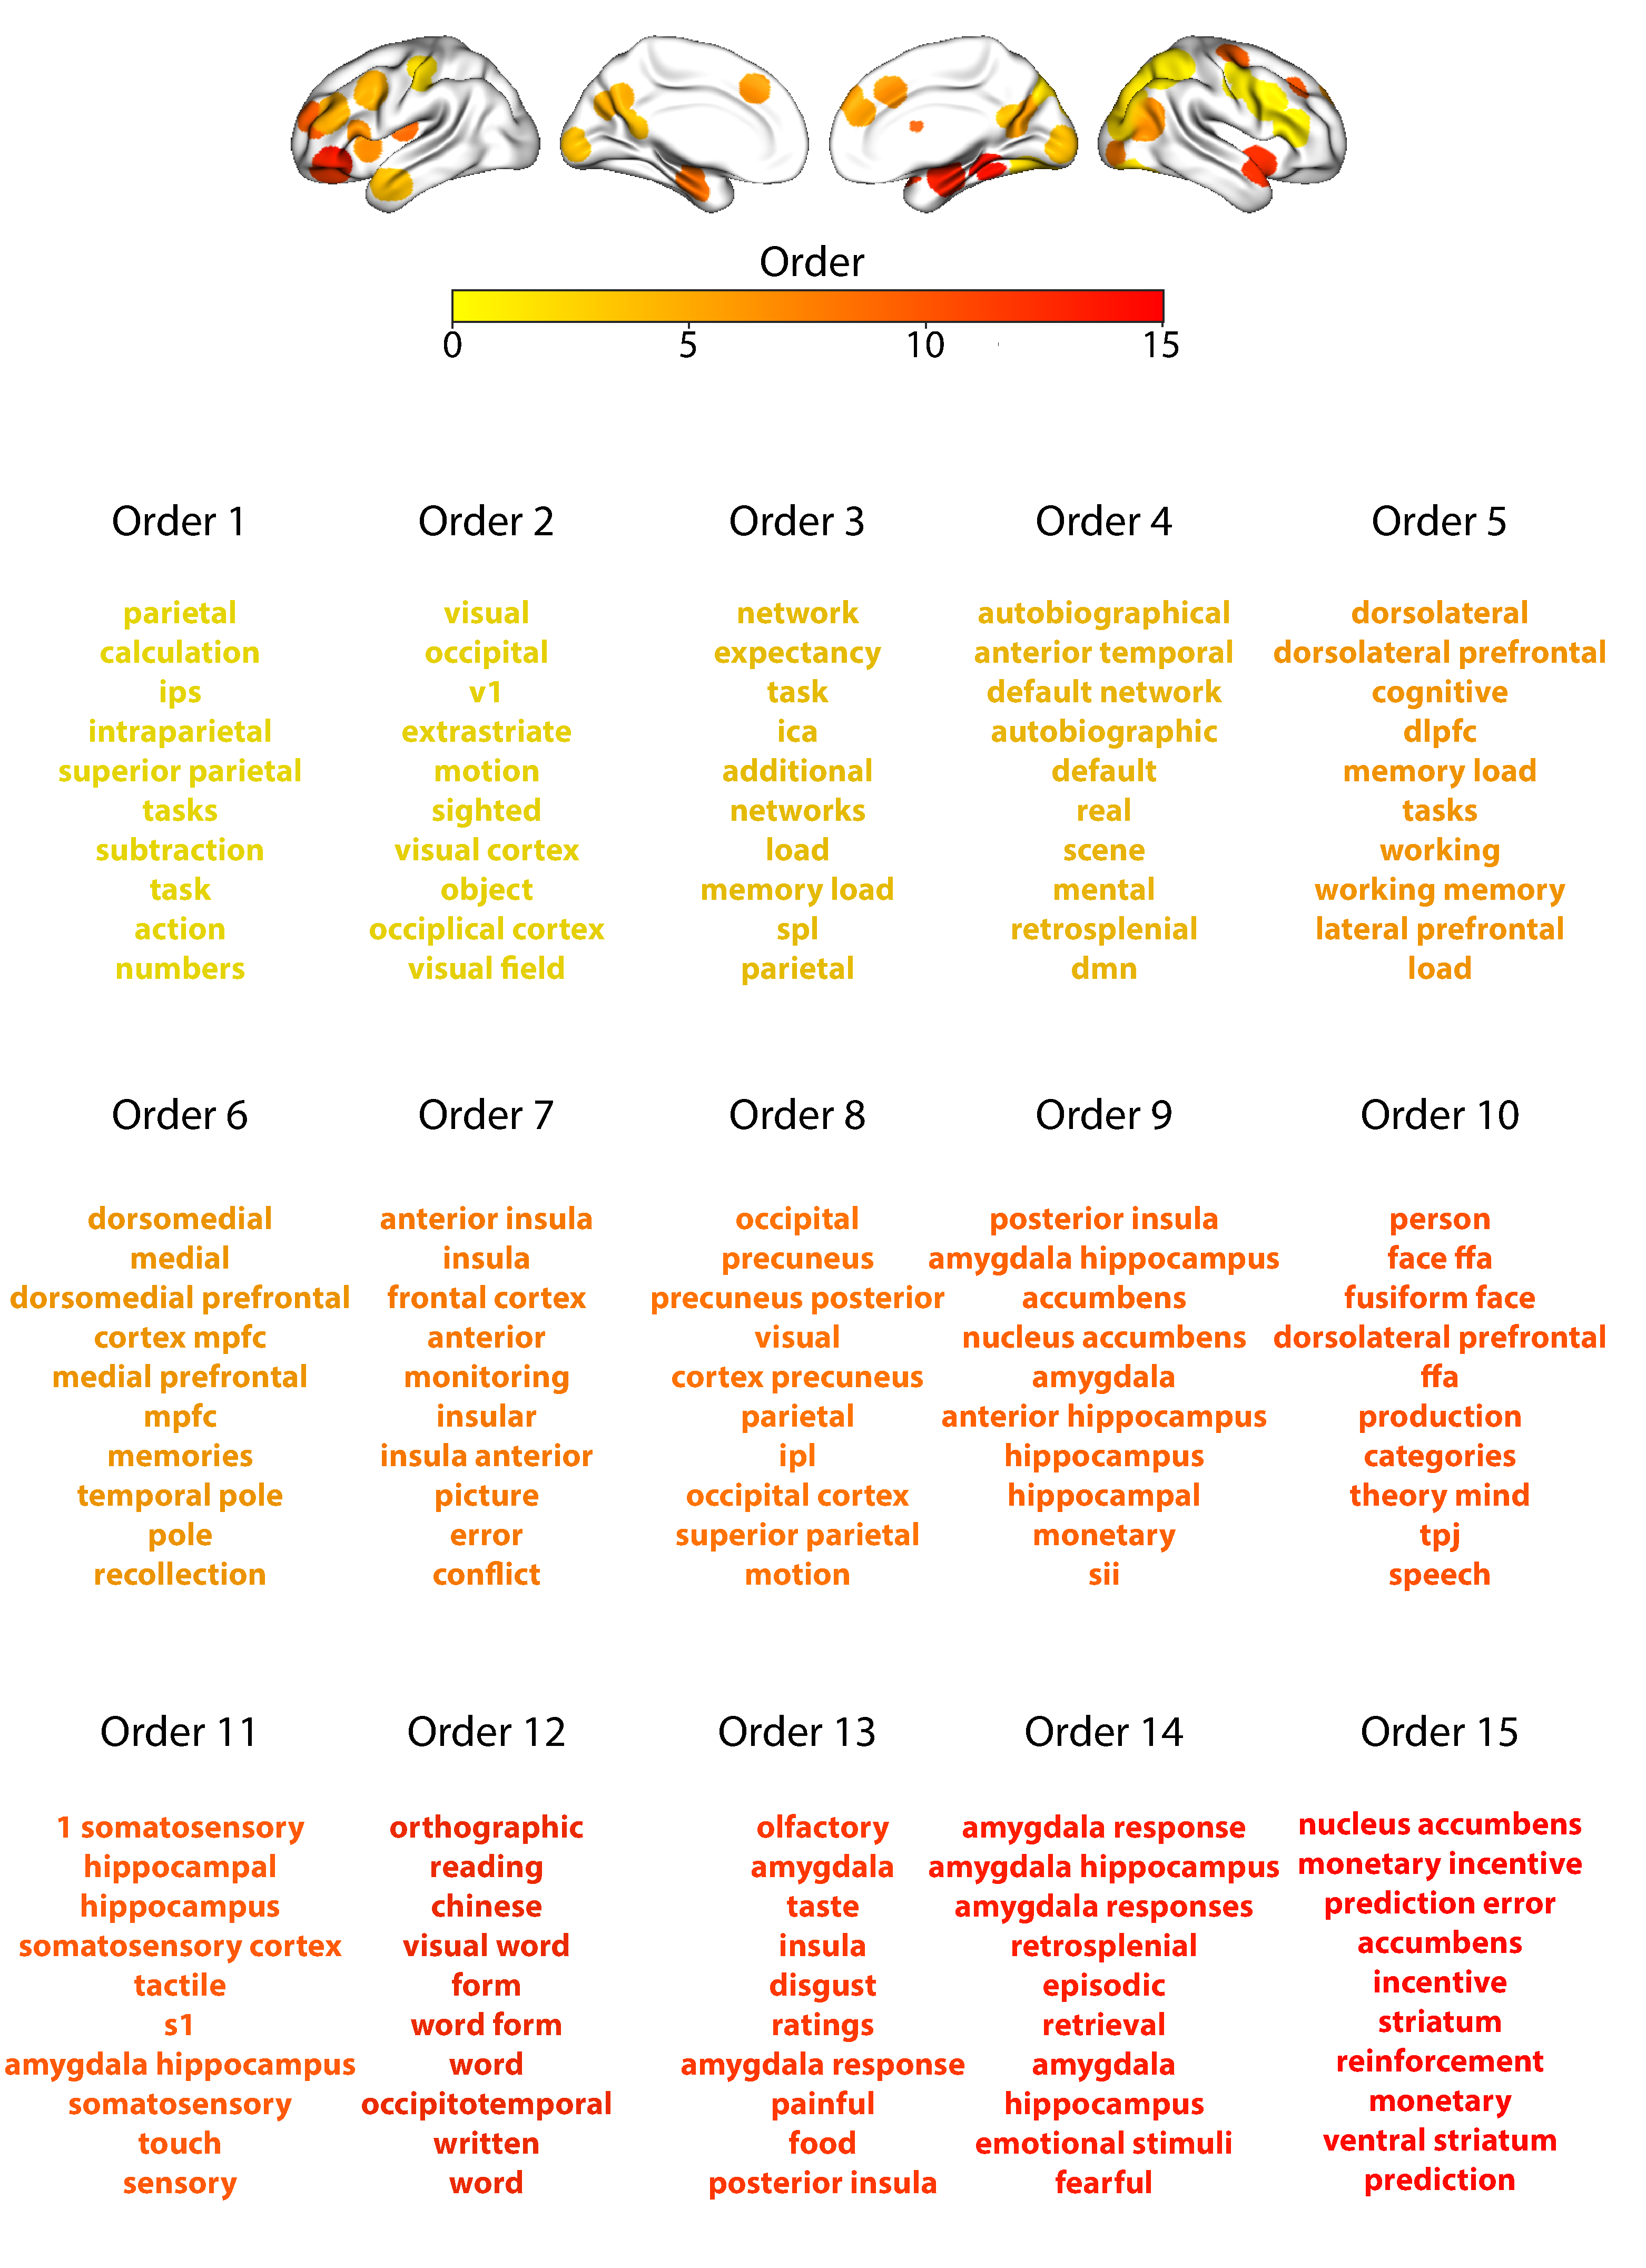
\includegraphics[width=0.75\textwidth]{figs/supp_15_rest}
\caption{\textbf{Top 10 terms associated with the endpoints of the
      strongest correlations for the rest condition.}  Each color corresponds to orders 1-15 of
    inter-subject functional correlations for the rest condition. The inflated brain plots
    display the locations of the endpoints of the 10 strongest
    (absolute value) correlations at each order, projected onto the
    cortical surface~\citep{CombEtal19}.  The lists of terms on the
    right display the top 10 Neurosynth terms~\citep{RubiEtal17}
    decoded from the corresponding brain maps for each order.}
\label{fig:rest}
\end{figure}



%\section*{Participant-level figures referenced in the main text}

% Supporting information


\newpage
\renewcommand{\refname}{Supplemental references}
\bibliography{memlab}


\end{document}